% One level of the Hybrid implementation (Section 3, Fig. fig:hybrid).
% Build: pdflatex diagram-final-opus.tex && cp diagram-final-opus.pdf ../../figs/approach-hybrid.pdf
\documentclass[tikz,border=2pt]{standalone}
\usepackage[T1]{fontenc}
\usetikzlibrary{arrows.meta,positioning,fit,backgrounds,shapes.geometric}
\begin{document}
\sffamily\footnotesize
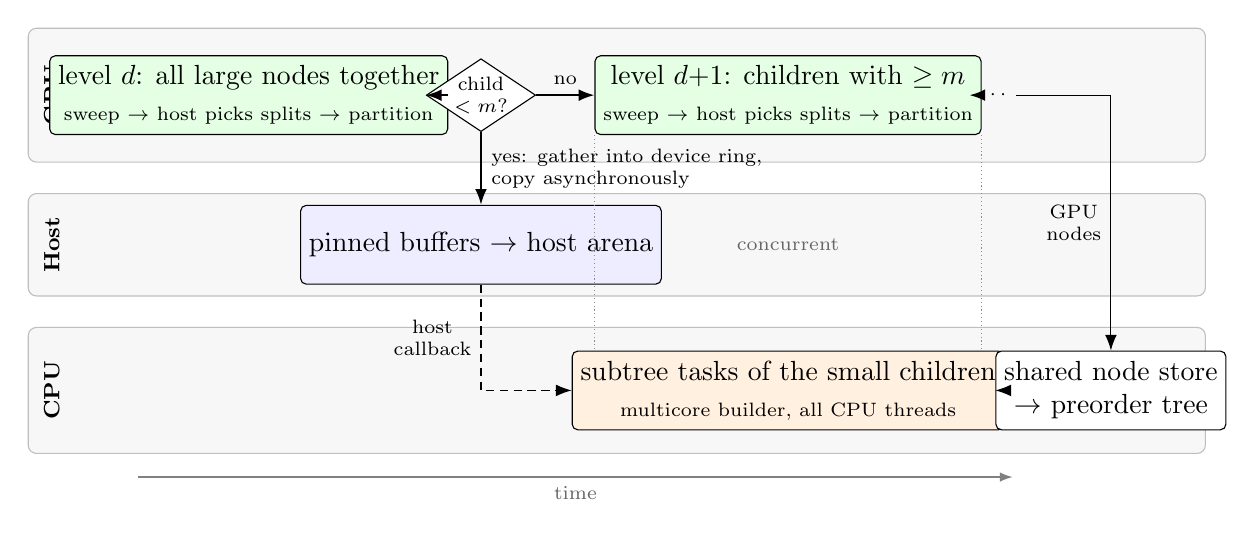
\begin{tikzpicture}[
  box/.style={draw, rounded corners=2pt, align=center, inner sep=3pt,
              minimum height=10mm},
  gpu/.style={box, fill=green!10},
  host/.style={box, fill=blue!7},
  cpu/.style={box, fill=orange!12},
  fork/.style={draw, diamond, aspect=1.5, inner sep=0pt, fill=white, align=center,
               font=\scriptsize},
  flow/.style={-{Latex[length=2mm]}, thick},
  small/.style={-{Latex[length=2mm]}},
  async/.style={-{Latex[length=2mm]}, densely dashed},
  lane/.style={draw=black!25, fill=black!3, rounded corners=3pt},
  lanelbl/.style={rotate=90, font=\bfseries\footnotesize},
  note/.style={font=\scriptsize, align=center}]

% ---------------- lanes ----------------
\begin{scope}[on background layer]
  \node[lane, fit={(-1.2, 0.85) (13.75,-0.85)}, inner sep=0] (Lg) {};
  \node[lane, fit={(-1.2,-1.25) (13.75,-2.55)}, inner sep=0] (Lh) {};
  \node[lane, fit={(-1.2,-2.95) (13.75,-4.55)}, inner sep=0] (Lc) {};
\end{scope}
\node[lanelbl] at (-0.9, 0)    {GPU};
\node[lanelbl] at (-0.9,-1.9)  {Host};
\node[lanelbl] at (-0.9,-3.75) {CPU};

% ---------------- GPU: level d, size test, level d+1 ----------------
\node[gpu, minimum width=37mm] (lvd) at (1.6,0)
  {level $d$: all large nodes together\\[1pt]
   \scriptsize sweep $\rightarrow$ host picks splits $\rightarrow$ partition};
\node[fork] (test) at (4.55,0) {child\\$<m$?};
\node[gpu, minimum width=37mm] (lvd1) at (8.45,0)
  {level $d{+}1$: children with $\ge m$\\[1pt]
   \scriptsize sweep $\rightarrow$ host picks splits $\rightarrow$ partition};
\node[note] (more) at (11.05,0) {$\cdots$};

\draw[flow] (lvd) -- (test);
\draw[flow] (test) -- node[above, note] {no} (lvd1);
\draw[flow] (lvd1) -- (more);

% ---------------- hand-off path ----------------
\node[host, minimum width=30mm] (arena) at (4.55,-1.9)
  {pinned buffers $\rightarrow$ host arena};
\draw[flow] (test) -- node[right, note, align=left]
  {yes: gather into device ring,\\copy asynchronously} (arena);

% ---------------- CPU pool, concurrent with level d+1 ----------------
\node[cpu, minimum width=52mm] (tasks) at (8.45,-3.75)
  {subtree tasks of the small children\\[1pt]
   \scriptsize multicore builder, all CPU threads};
\draw[async] (arena.south) |- node[pos=0.25, left, note] {host\\callback} (tasks.west);

% concurrency marker: dotted guides from level d+1 down to the tasks
\draw[black!45, densely dotted] (lvd1.south west) -- (tasks.north west -| lvd1.south west);
\draw[black!45, densely dotted] (lvd1.south east) -- (tasks.north east -| lvd1.south east);
\node[note, text=black!60, fill=black!3] at (8.45,-1.9) {concurrent};

% ---------------- one tree ----------------
\node[box, fill=white, minimum width=24mm] (store) at (12.55,-3.75)
  {shared node store\\$\rightarrow$ preorder tree};
\draw[small] (tasks) -- (store);
\draw[small] (more.east) -| node[pos=0.75, left, note] {GPU\\nodes} (store.north);

% ---------------- time ----------------
\draw[-{Latex[length=1.6mm]}, black!50] (0.2,-4.85) -- node[below, note, text=black!60] {time} (11.3,-4.85);
\end{tikzpicture}
\end{document}
